\documentclass[../main.tex]{subfiles}
\graphicspath{{\subfix{../figures/}}}
\begin{document}
The theory part of the thesis is divided into three sections. Firstly, a brief overview of the theory behind transport through quantum dots is given. Then, the focus is turned to some of the tools used in open quantum systems, ultimately ending in a section about quantum master equations. The final section will further explain the notion of exceptional points, and introduce a couple of important tools used in exceptional point physics.

\section{Transport through quantum dots}
To begin understanding the transport of electrons through a system of quantum dots, it is insightful to first study the single quantum dot system. The following explanation is inspired by reference~\cite{transport}.

Consider a single quantum dot with $N$ electrons capacitively coupled to a gate and coupled to source and drain reservoirs through tunnel junctions as in \cref{fig:qdotscheme}. The main transport properties of the system can then be understood in terms of the chemical potentials of the quantum dot and the source and drain reservoirs. These are often depicted in electro-chemical potential diagrams, see \cref{fig:ladder}. There, $\mu(N)$ is the energy required to add the $N$th electron to the quantum dot, and $\mu_S$ and $\mu_D$ are the Fermi levels of the source and drain. The shaded areas represent the Fermi-Dirac distributions of the reservoirs.
\begin{figure}[H]
    \centering
    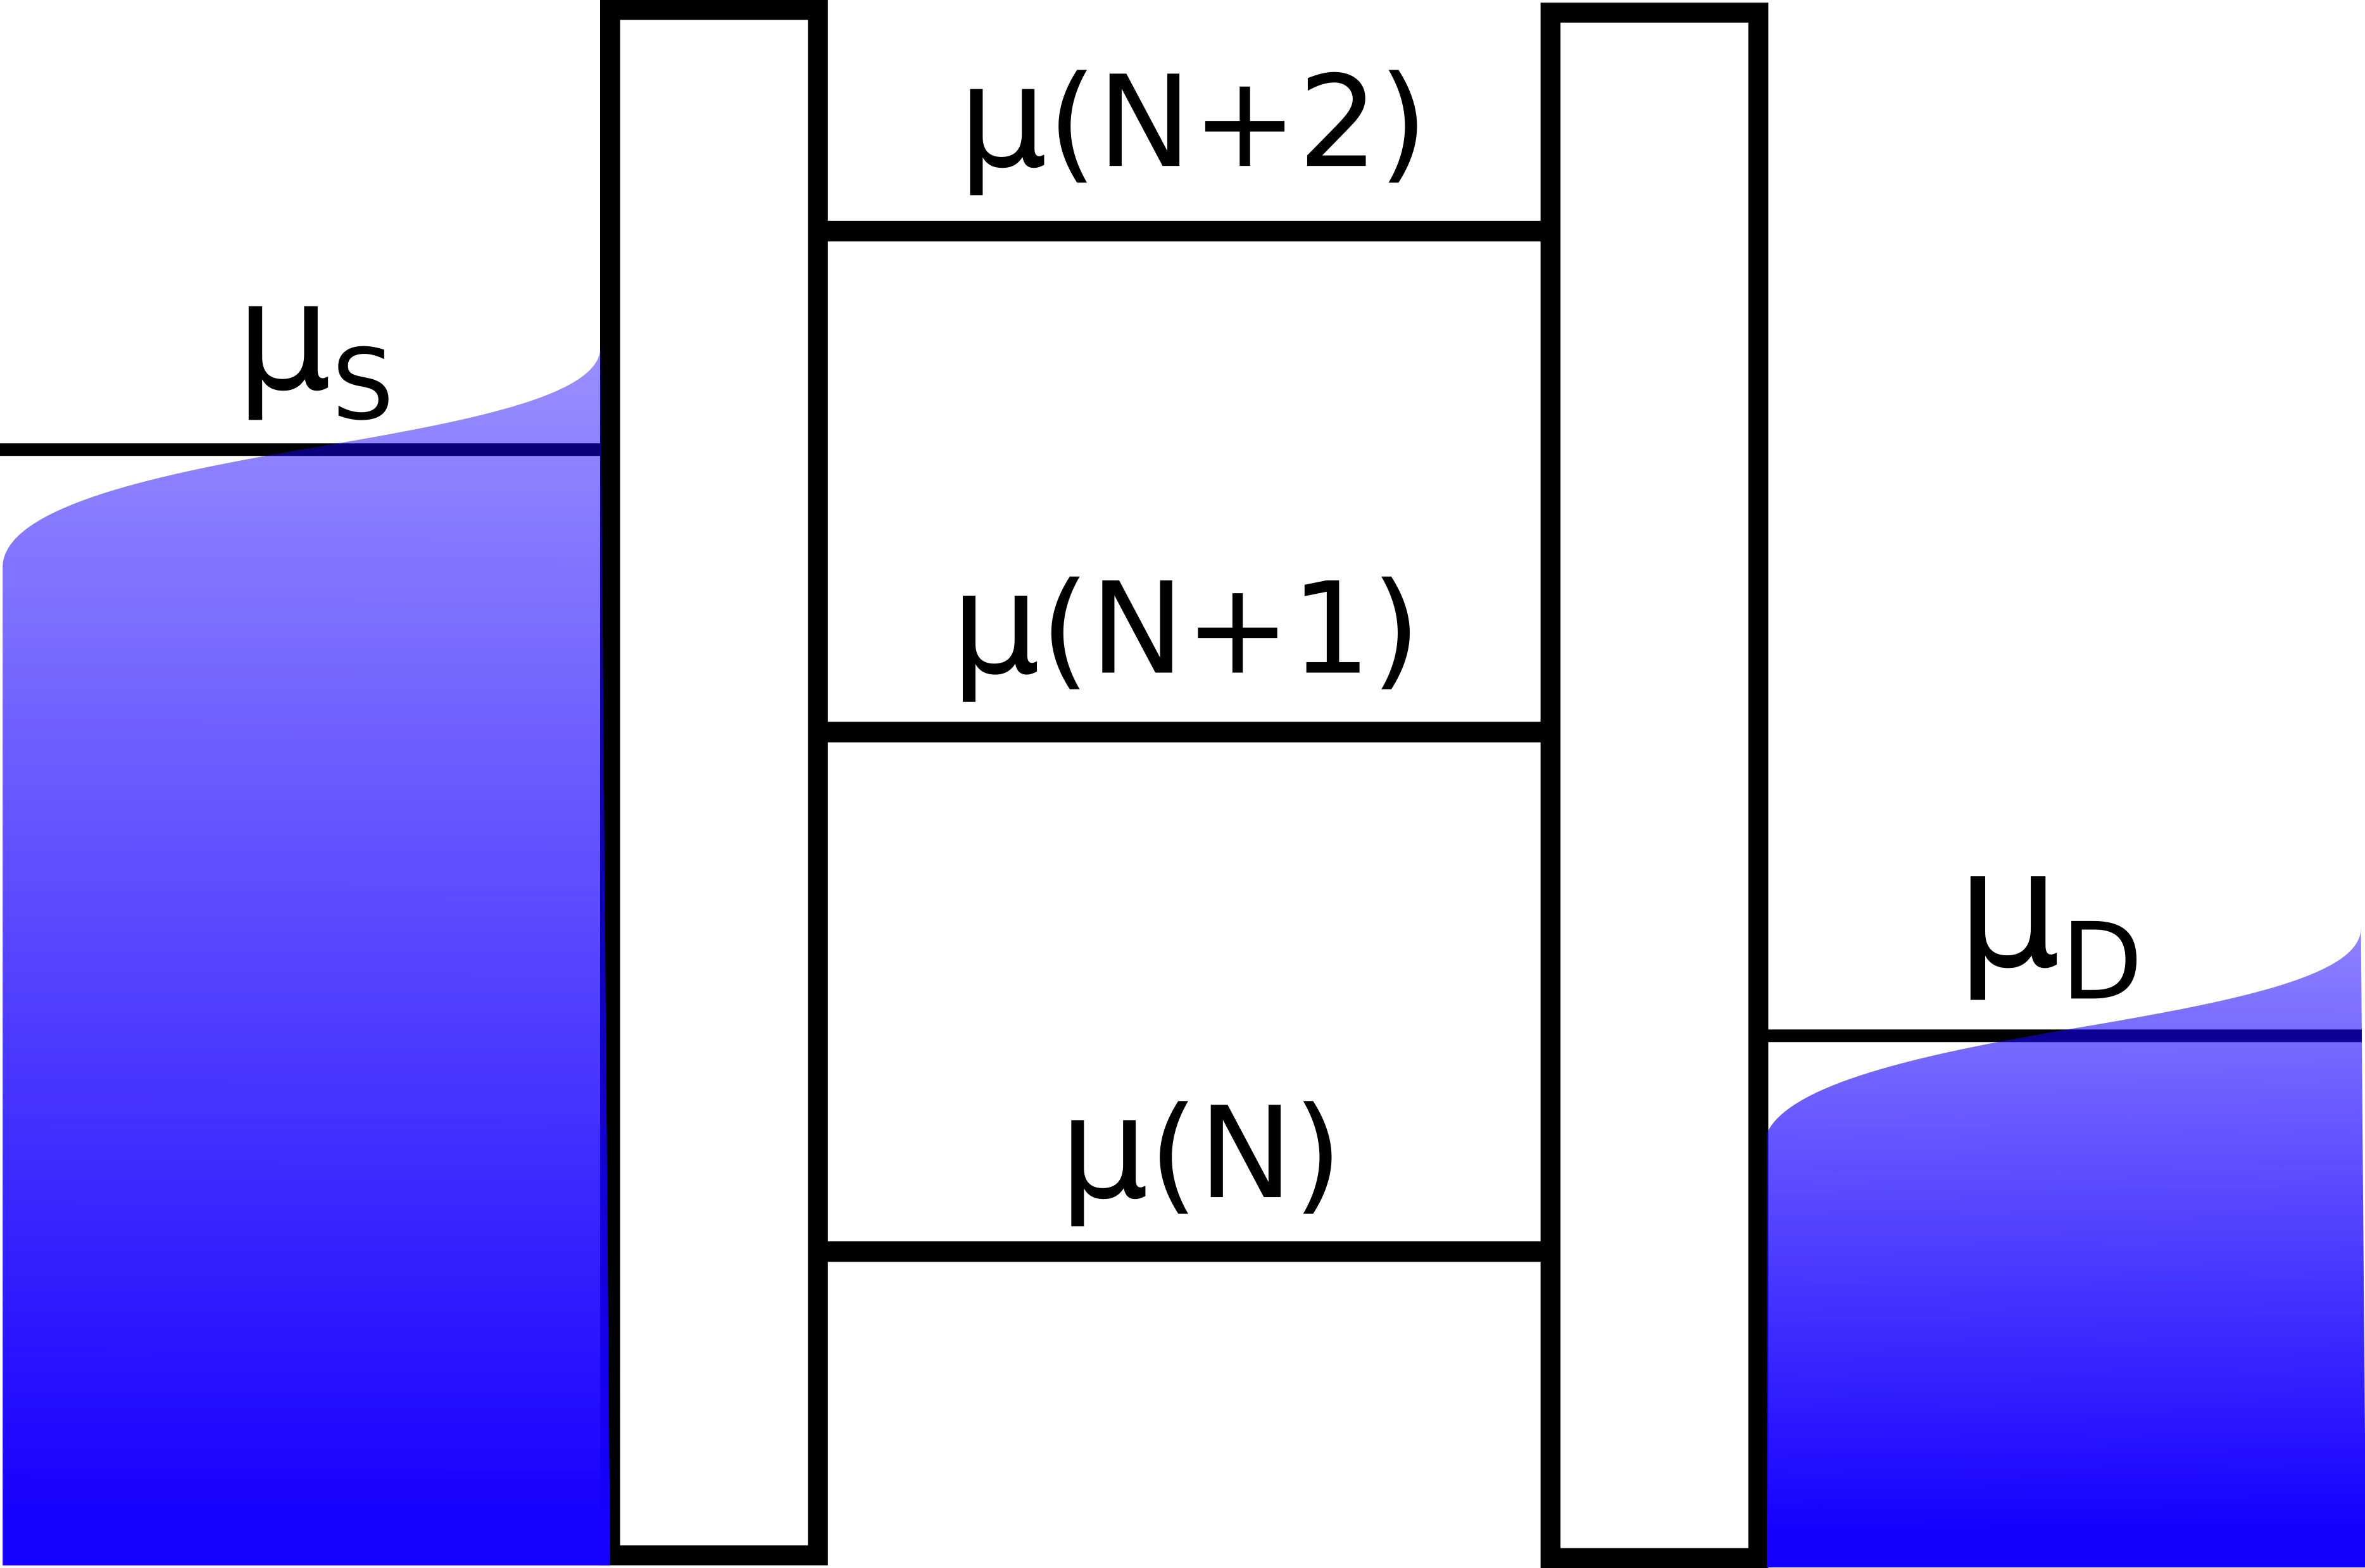
\includegraphics[width=0.5\linewidth]{figures/ladder.png}
    \caption{An electro-chemical potential diagram of the single quantum dot system. The source and drain are in a thermal distribution given by the shaded areas with Fermi levels $\mu_S$ and $\mu_D$. The quantum dot is depicted as a ladder with energies $\mu(N)$, representing the energy required to add the $N$th electron to the dot.}
    \label{fig:ladder}
\end{figure}
Using this picture, the electron transport through the quantum dot can be easily visualized. If the chemical potential levels are located as in \cref{fig:ladder}, $\mu(N + 1)$ is below $\mu_S$, and an electron will likely tunnel from the source onto the dot, increasing the number of electrons on the dot from $N$ to $N+1$. After the tunneling event, there is an even lower chemical potential available for the electron, $\mu_D$, and the electron will with a high probability leave the quantum dot and enter the drain. In this fashion, the system will cycle through having $N$ and $N+1$ electrons on the dot, producing a current.  

It turns out that $\mu(N)$ depends linearly on the gate voltage $V_G$, so by changing it, the ladder of states in \cref{fig:ladder} can be lowered or raised. The source-drain voltage $V_{SD}$ on the other hand, changes the distance between $\mu_S$ and $\mu_D$. Through these two processes, it is possible to change the electro-chemical potential landscape and therefore control the current through the system. This captures the main behavior of the dynamics of the quantum dot system. However, by adapting the theory of open quantum systems, a much richer and more accurate theory can be developed.

\section{The theory of open quantum systems}
Open quantum systems are systems which are non-isolated and connected to some sort of environment. Often, it considers a total system consisting of the (sub)system of interest, and an environment. The total system is closed, and therefore it obeys the standard quantum mechanical equations of motion. The goal of the theory of open quantum systems is to infer the dynamics of the smaller system from the equations of the total system~\cite{lindblad}. To do this, a few fundamental tools used in this field need to be introduced.

\subsection{The von Neumann equation and the reduced density operator}

An essential tool used in the theory of open quantum systems is the density operator $\hat{\rho}$. In such systems, the exact state of the system is generally unknown. Instead, the system may be known to be in a state $\ket{\psi_k}$ with a probability $p_k$, or in another state $\ket{\psi_l}$ with a different probability $p_l$. Generally, the system is then said to be in an ensemble $\{\ket{\psi_k}, p_k\}_k$. The density operator describes this information in a compact way:
\begin{equation}
    \hat{\rho} = \sum_k p_k \ket{\psi_k}\bra{\psi_k}.
\end{equation}
It can easily be shown that the density operator is Hermitian and has unity trace. Furthermore, by fixing a basis $\{\ket{\phi_i}\}$, the density operator can be represented by its matrix elements 
\begin{equation}
    \rho_{ij} = \braket{\phi_i|\hat\rho|\phi_j} = \sum_k p_k \braket{\phi_i|\psi_k}\braket{\psi_k|\phi_j}.
\end{equation}
The diagonal elements $\rho_{ii}$ represents classical probabilities of being in a state $\ket{\phi_i}$ and the off-diagonal elements $\rho_{ij}$ are the so called coherences between state $\ket{\phi_i}$ and $\ket{\phi_j}$. Note that the matrix elements are basis dependent, and that there always is a basis in which the density operator is diagonal~\cite{bookopen}.

The average measured value of an observable $\hat O$ of an ensemble represented by $\hat\rho$ is given by
\begin{equation}\label{eq:expec}
    \braket{\hat O} = \tr({\hat\rho \hat O}).
\end{equation}
From the density operator one can therefore extract all signifiant information from the ensemble, and it can be described as the "state" of the system. It is also possible to calculate how the density operator evolves over time. Under a Hamiltonian $\hat H$, the evolution is given by the von Neumann equation
\begin{equation}\label{vonneumann}
    i\hbar\diff{\hat\rho}{t} = [\hat H, \hat\rho] \equiv \mathcal{L}\hat\rho,
\end{equation}
where $\mathcal{L}$ is the Liouvillian superoperator, or just the Liouvillian~\cite{bookopen}. 

The Liouvillian $\mathcal{L}$ in \cref{vonneumann} is an operator acting on an operator, hence being called a superoperator. However, it is possible to treat it as a normal operator which acts on a Hilbert space spanned by the density matrices. The Liouvillian can therefore be represented by a matrix $L$, which acts on a vector representation of the density matrices, usually written as $\ket{\rho}\rangle$. The Hilbert space spanned by these vectors is called the Fock-Liouville space, equipped with a scalar product $\langle\braket{\rho_1|\rho_2}\rangle$~\cite{lindblad}. 

Returning to the mentioned goal of the theory of open quantum systems, a natural question is the following:How do we extract the density operator of a subsystem $\hat\rho_S$, from the total density operator $\hat\rho_T$, the latter describing the closed, full system? This question is resolved by the reduced density operator. If the total system $T$ consists of a subsystem $S$ and an environment $E$, then the reduced density matrix for the subsystem is given by
\begin{equation}
    \hat\rho_S = \tr_E({\hat\rho_T}),
\end{equation}
where $\tr_E$ is the partial trace over the environment. The partial trace essentially takes the average with respect to the environmental degrees of freedom. This way, a density operator for the subsystem of interest is obtained without having to simulate the whole system. The reduced density operator contains all measurement statistics of interest in the subsystem, placing it at the core of the theory of open quantum systems~\cite{bookopen}.

\subsection{The Lindblad Master equation}\label{sec:lind}
An important framework for determining the dynamics of an open quantum system is the master equation approach. A classical master equation is defined by
\begin{equation}\label{master}
    \diff{p_i}{t} = \sum_j R_{ji}p_j  - \sum_j R_{ij}p_i,
\end{equation}
with probabilities $p_i$ of being in state $\ket{\psi_i}$, and transition rates $R_{ij}$ describing the rate of transitions from $\ket{\psi_i}$ to $\ket{\psi_j}$. As an example, the states in a quantum dot system may correspond to the number of electrons on the dot while the transition rates are typically related to the Fermi-Dirac distributions of the reservoirs and the tunneling rates of the barriers~\cite{transport}.

Collecting the rate equations for each $i$ and adding the condition $\sum_i p_i = 1$ such that the total probability is unity, a system of ordinary differential equations is obtained. This can be solved numerically using standard methods for first order differential equations, such as the Runge-Kutta method~\cite{iserles}. Once the probabilities are obtained, the evolution of the current can be calculated by considering the amount of charge tunneling through the barriers at each point in time~\cite{transport}.

While a classical master equation may give accurate results for some quantum systems, it leaves out important physics. A quantum master equation generalizes the notion of a classical master equation in the following sense: The unknown in a quantum master equation does not only contain the probabilities $p_i$ of being in a quantum state $\ket{\psi_i}$, but also the coherences. Hence, a quantum master equation involves the full density matrix while a classical master equation only includes the diagonal elements. However, since it always is possible to find a basis such that the density matrix is diagonal, the two master equations can be equivalent in certain bases.

The starting point for quantum master equations is \cref{vonneumann}, the von Neumann equation, for the density matrix of the total system. Using the partial trace, a differential equation for the reduced density matrix (from now on written as $\hat\rho$) of the system of interest can be obtained. However, the resulting equation still includes the total density operator and approximations have to be made~\cite{lindblad}. One common approximation is to assume that the coupling between the system and the environment is weak in comparison to the other energy scales of the system. This way, the interaction can be treated perturbatively, and progress can be made. One of the most established quantum master equations, the Lindblad equation, is derived in this fashion~\cite{lindorigin}, and is given by
\begin{equation}\label{eq:lind}
    \diff{\hat\rho}{t} = i[\hat\rho, \hat H_\text{eff}] + \sum_i \hat L_i\hat\rho\hat L_i^\dag - \frac{1}{2}\hat\rho\hat L_i^\dag\hat L_i - \frac{1}{2}\hat L_i^\dag\hat L_i \hat\rho \equiv \mathcal{L}\hat\rho,
\end{equation}
where $\hat H_\text{eff}$ is the sum of two terms: the subsystem Hamiltonian $\hat H_\text{S}$ and the Lamb shift Hamiltonian $\hat H_\text{LS}$, a renormalization of energy levels due to the interaction with the environment~\cite{lindblad}. The operators $\hat L_i$ are the so called jump operators, which capture the coupling processes to the environment. In Ref.~\cite{perlind}, a phenomenological approach for calculating the jump operators is described. Using this so called PERLind approach, the jump operators are (something). Once the jump operators are constructed and the first term of \cref{eq:lind} is calculated, an expression for the Liouvillian $\mathcal{L}$ can be obtained. 

The right hand side of the Lindblad equation can be divided into two parts. The first term, $i[\hat\rho, \hat H_\text{eff}]$, describes the unitary, free evolution of the system. A simple example of a free evolution would be the precession of magnetic moment in a magnetic field. The sum over $i$ on the other hand, correspond to the non-unitary and dissipative part of the dynamics~\cite{bookopen}. The latter part causes the total Liouvillian to be non-Hermitian, which brings the possibility of exceptional points in the matrix representation of the Liouvillian. EPs in the Liouvillian superoperator lead to signatures in the dynamics of the density operator. This will be further developed in the next section.  

%One of the attractive properties of the Lindblad equation is that it ensures the positivity and unity trace of the density operator throughout the evolution (explain in prev section). Other quantum master equations do not have this property, which may cause negative probabilities and other unphysical results.

\section{Exceptional points}\label{sec:ep}
A matrix which describes the evolution of a physical system, such as a Hamiltonian or a Liouvillian matrix, generally depends on the parameters of the system. These parameters span the so called parameter space, and it is in this space the exceptional points lie. An exceptional point is defined as a point in the parameter space which causes two or more eigenvalues and their eigenvectors to simultaneously coalesce~\cite{nonHermrev}. An EP is said to be of a certain order, reflecting how many eigenvectors coalesce at the point. The notion of exceptional points and its orders are directly related to a type of matrix decomposition, the Jordan normal form.

\subsection{Jordan normal form}

In physics, a common way to simplify calculations is to diagonalize the matrix generating the evolution of the system. The diagonalization process can be understood a change of basis to linearly independent eigenvectors. In this basis, the linear transformation of the matrix is very simple: it scales each eigenvector $r_i$ by the corresponding eigenvalue $\lambda_i$. The matrix in the new basis is therefore diagonal, explaining the name of the process. For a matrix $A$ and its diagonal form $D$, this can be written as 
\begin{equation}
    A = SDS^{-1},
\end{equation}
where $S = (r_1, \dots ,r_n)$ consists of the eigenvectors of $A$, obeying $Ar_i=\lambda_ir_i$~\cite{uffe}.

However, not all matrices can be diagonalized, the exceptions being called defective matrices. For a defective matrix, there does not exist a basis of eigenvectors, and the diagonalization process is not possible~\cite{uffe}. This is closely related to the notion of exceptional points, since when two eigenvectors coalesce, one dimension is lost and the eigenvectors do not form a basis anymore. A matrix at an EP is therefore always defective.

Fortunately, there is a notion of an "almost diagonal" form for defective matrices, called the Jordan normal form. Recall that in the diagonalizable case, the basis is changed to the linearly independent eigenvectors. To construct the Jordan form for a defective matrix, this basis has to be completed in some way to span the full space. This can be done using Jordan chains~\cite{uffe}, which for each eigenvector $r_i$ with eigenvalue $\lambda_i$, consist of vectors $r_i, r_i^{(2)}, \dots,   r_i^{(n_i)}$ defined by
\begin{equation}\label{jordanchain}
\begin{aligned}
    (A-\lambda_iI)r_i &= 0 \\
    (A-\lambda_iI)r_i^{(2)} &= r_i \\
    (A-\lambda_iI)r_i^{(3)} &= r_i^{(2)} \\
    &\;\;\vdots \\
    (A-\lambda_iI)r_i^{(n_i)} &= r_i^{(n_i-1)},
\end{aligned}
\end{equation}
where $I$ is the identity matrix. These vectors are also known as generalized eigenvectors. The length of the $i$th chain, $n_i$, depends the number of coalescing eigenvectors, and is therefore the same as the order of the corresponding EP. Note that for eigenvectors not involved in an EP, i.e., for eigenvectors which have not coalesced, the Jordan chain is of length one, only consisting of the eigenvectors themselves. Creating these chains for each linearly independent eigenvector results in $q$ Jordan chains, each of which are collected into the matrices
\begin{equation}
    \{\boldsymbol{r}_i\}_{i=1}^q, \text{ where }\boldsymbol{r}_i = (r_i, r_i^{(2)},\dots ,r_i^{(n_i)}).
\end{equation}
Here, the bold font indicates a collection of column vectors next to each other, forming a matrix. The collection of generalized eigenvectors from all Jordan chains is called the canonical basis of the transformation. Using this new basis, the matrix $A$ can be transformed into its Jordan form $J$ with the transformation matrix 
\begin{equation}\label{chofba}
    M = (\boldsymbol{r}_1, \dots, \boldsymbol{r}_q),
\end{equation}
which also is known as the modal matrix. The Jordan normal form of $A$ is then obtained by forming $J = M^{-1}AM$ and has the following structure: 
\begin{equation}\label{eq:jordan}
    J = \begin{bmatrix}J_{n_1}(\lambda_1) & \dots & 0 \\
                            \vdots & \ddots & \vdots \\
                        0 & \dots &  J_{n_q}(\lambda_q)\end{bmatrix}, \text{ where }
       J_{n_i}(\lambda_i) = \begin{bmatrix} \lambda_i & 1 & \dots & 0 \\
                                                    \vdots  & \ddots & \ddots & \vdots \\
                                                    \vdots & & \ddots& 1 \\
                                                    0 & \dots & \dots & \lambda_i\end{bmatrix}.
\end{equation}
The Jordan form hence consists of $q$ Jordan blocks $J_{n_i}(\lambda_i)$ on the diagonal, where each block is of size $n_i$ and consists of its eigenvalue on the diagonal and ones on the super diagonal~\cite{uffe}. Note that if all blocks are of size one, i.e., there are no exceptional points, the Jordan form is diagonal. The Jordan normal form can therefore be thought of a generalization of the diagonal form $D$.

A simple example of the construction of a Jordan normal form is helpful to understand the process.

Unfortunately, the Jordan form of a matrix is notoriously difficult to calculate numerically. This stems from the fact that an arbitrary small perturbation away from an EP completely changes the Jordan form. The process is therefore inherently numerically unstable. For simple cases, it is however possible to work around this difficulty. By introducing a small tolerance to determine if eigenvalues and their eigenvectors have coalesced, one can then infer the block structure of the Jordan form and construct it manually.

To be able to use the Jordan form in calculations, a substitution $A\rightarrow MJM^{-1}$ has to be made, and hence, the matrices $M$ and $M^{-1}$ are also desirable to compute. The matrix $M$ consists of the generalized eigenvectors, which can be calculated by the following process. Firstly, the regular eigenvectors are calculated by some numerical method, e.g., the \verb+numpy.linalg.eig+ function in Python. If there are coalesced eigenvectors, the corresponding Jordan chains need then to be computed. This can be done by solving the defining equations for the generalized eigenvectors given by \cref{jordanchain}. However, since $A-\lambda_iI$ is not of full rank, the equations are underdetermined, meaning that there does not exist a unique solution. A standard way of solving this problem is by using the Moore-Penrose pseudoinverse, which finds one of the solutions to the equation~\cite{uffe}. This process is then repeated until the full Jordan chains for each set of coalescing eigenvectors are calculated, obtaining all of the generalized eigenvectors and hence, the modal matrix $M$. 

A straightforward way of calculating the inverse modal matrix $M^{-1}$, is just to numerically invert $M$. However in the literature regarding Liouvillian exceptional points, the rows in $M^{-1}$ is often referred to as the \textit{left} generalized eigenvectors. Explain what they are. These can be constructed biorthonormally to the regular generalized eigenvectors, effectively creating $M^{-1}$. The left generalized eigenvectors can be numerically calculated by a similar method as the right ones. However, these then have to be modified such that they are orthogonal to the right generalized eigenvectors, which can be done using LU-decomposition. We now turn our attention to a useful application of the Jordan normal form, ODEs.

\subsection{General solution of ODEs}
An ordinary differential equation (ODE) is a linear differential equation of the form
\begin{equation}\label{eq:ode}
    \diff{x}{t}=Ax. 
\end{equation}
Often, the unknown $x$ is a vector, and $A$ a matrix. The solution can then be written as a matrix exponential in the following way:
\begin{equation}
    x(t) = e^{At}x(0), \;\text{where } \;e^{At} = \sum_{k=0}^{\infty}\frac{(At)^k}{k!}.
\end{equation}
The matrix exponential can be simplified using Jordan decomposition. It can be shown that  $e^{At} = Me^{Jt}M^{-1}$ where $M$ is the modal matrix and
\begin{equation}\label{eq:expjordan}
        e^{Jt} = \begin{bmatrix}e^{J_{n_1}(\lambda_1)t} & \dots & 0 \\
                                                         \vdots & \ddots & \vdots \\
                                                         0 & \dots &  e^{J_{n_q}(\lambda_q)t}\end{bmatrix}, \text{ where } 
            e^{J_{n_i}(\lambda_i)t} = e^{\lambda_it} \begin{bmatrix} 1 & t & \dots & \frac{t^{n_i-1}}{(n_i-1)!}\\
                                                                \vdots  & \ddots & \ddots & \vdots \\
                                                                \vdots & & \ddots& t \\
                                                            0 & \dots & \dots & 1\ \end{bmatrix}.
\end{equation}
The matrix exponential therefore consists of entries with terms of the form $t^ke^{\lambda_it}$~\cite{uffe}. Note that if $A$ is diagonalizable, all blocks are of size one and the entries consist of pure exponentials on the diagonal. 

Using this result, the solution to \cref{eq:ode} can be written as 
\begin{equation}\label{jordanode}
    x(t) = Me^{Jt}M^{-1}x(0).
\end{equation}
This can further be decomposed if one considers the generalized modes of the system. A generalized mode in this context is meant as the solution to the ODE, with an initial condition in a linear combination of vectors in \textit{one} of the Jordan chains. It can be shown that the trajectory then never leaves that Jordan chain throughout the whole evolution.

To show this, suppose first that the initial state is in such an initial state, i.e., a linear combination of vectors in one of the Jordan chains:
\begin{equation}
    x(0) = a_1r_i + a_2r_i^{(2)} + \dots + a_{n_i}r_i^{(n_i)} = \boldsymbol{r}_ia,
\end{equation}
where $a = (a_1, \dots a_{n_i})^T$ is a constant vector and $\boldsymbol{r}_i$ is defined in \cref{chofba}. Then we rewrite $M^{-1}$ as
\begin{equation}
    M^{-1} = \begin{bmatrix} \boldsymbol{l}_1 \\ \vdots \\ \boldsymbol{l}_{q} \end{bmatrix},\end{equation}
    where $\boldsymbol{l}_i$ contain $n_i$ row vectors. Since $M^{-1}M=I$, it follows that $\boldsymbol{l}_j \boldsymbol{r}_i = \delta_{ij}I$ where $I$ is the $n_j\times n_i$ identity matrix. Inserting this into \cref{jordanode}, the solution can be written as
\begin{equation}\label{eq:genmode}
    x(t) = Me^{Jt}M^{-1}x(0) = Me^{Jt} \begin{bmatrix} \boldsymbol{l}_1 \\ \vdots \\ \boldsymbol{l}_{q} \end{bmatrix} \boldsymbol{r}_ia = \boldsymbol{r}_i e^{J_{n_i}(\lambda_i)t} a.
\end{equation}
Hence, the solution stays in the space spanned by the initial condition throughout the evolution, as earlier proposed. For an arbitrary initial condition, the solution can be written as a sum over the generalized modes: 
\begin{equation}
    x(t) = \sum_{i=1}^q \boldsymbol{r}_i e^{J_{n_i}(\lambda_i)t} \boldsymbol{l}_i x(0).
\end{equation}
Translating this theory into the language of Liouvillian physics, the underlying ODE is given by the Lindblad equation, transformed to Fock-Liouville space    
\begin{equation}
    \diff{\rho(t)}{t}= \mathcal{L} \rho(t) \rightarrow \diff{}{t}\ket{\rho(t)}\rangle = L \ket{\rho(t)}\rangle,
\end{equation}
where $L$ is the matrix representation of the Liouvillian and $\ket{\rho(t)}\rangle$ the vectorized density matrix. Using \cref{eq:genmode}, the solution can then be written in terms of the eigenvalues and generalized eigenvectors of $L$. \Cref{eq:genmode} is very general since it can be used for any orders of the EP, including when the system is not at an exceptional point.

% \begin{equation}\label{eq:genmodeFL}
%     \ket{\rho(t)}\rangle = \sum_{i=1}^q \begin{bmatrix} \ket{\rho_i}\rangle, & \ket{\rho_i'}\rangle, & \ket{\rho_i''}\rangle, & \dots \end{bmatrix} e^{J_{n_i}(\lambda_i)t} \begin{bmatrix} \langle\bra{\sigma_i} \\ \langle\bra{\sigma_i'}\\ \langle\bra{\sigma_i'' } \\ \vdots \end{bmatrix}\ket{\rho(0)}\rangle.
% \end{equation}
% Here, $\ket{\rho_i}\rangle, \ket{\rho_i'}\rangle, \ket{\rho_i''}\rangle, \dots$ are the generalized eigenvectors of $L$ and $\langle\bra{\sigma_i}, \langle\bra{\sigma_i'}, \langle\bra{\sigma_i'' }, \dots$ the corresponding rows in $M^{-1}$.


\end{document}






